\addtocontents{toc}{\protect\setcounter{tocdepth}{0}}
\addtotoc{Management Summary}
\chapter*{Management Summary}
The standardization of technology communication protocols is nowadays mandatory in our current world of emerging technology. Geospatial information and services related to it have been growing a lot over the few years. And with this happening, the need for standardization of such geospatial services has been rising as well. An important organization for standardizing such services is The \href{https://www.ogc.org/}{\textit{Open Geospatial Consortium (OGC)}} consortium. This international consortium consists of a lot of businesses, organizations and universities that contribute into standardizing the geospatial information and services.\\
In this project, we try to comply with one of the OGC standards called the \href{https://docs.opengeospatial.org/is/17-069r3/17-069r3.html}{\textit{OGC API - Features}} standard. It is a standard that specifies the behaviour of Web APIs that provide access to geospatial features in a dataset. It contains discovery operations and query operations. Discovery operations show the capabilities of the Web API and the distribution of it's dataset, while on the other hand, query operations enable the clients to retrieve features from the underlying data set based on criterias, that are of course defined by the client.
\section*{Goals}
The main goals for this application is to create an API that is minimally compliant with the \textit{OGC API - Features (OAPIF)} standard. The \textit{Geospatial Data Abstraction Library (GDAL)} is a computer software library for reading and writing raster and vector geospatial data formats. The importance of this library here is that this application also supports some other responses for one of the GDAL drivers which is called the \textit{OAPIF} driver, it is a driver that is developed by GDAL in order to communicate with OAPIF APIs.
The application initially expects one or more GeoJSON files (called layers),
containing a feature collection as initial input for the API. It then processes this data and manipulates with it in order to give the correct API responses.\\
This application also has to be able to be integrated with the experimental QGIS \textit{WFS3} vector layer feature which queries the given API and adds the feature collection of the application into the QGIS map. Another requirement for this application is to be operable by the \textit{ogrinfo} program, which is a program contained in the GDAL library that lists information about a data source that is supported by GDAL. In this case, the ogrinfo program must be able to make requests to this application and receive correct responses from it using the OAPIF driver
\section*{Results}
This API has been tested with the OAPIF GDAL driver using the ogrinfo
command-line tool in order to test if this driver can successfully communicate with the API and if it is able to, it would mean that this API is minimally compliant with the OGC API - Features standard. This test was completed with success. The application has also been tested with an existing OAPIF client, in where it serves as an API to this application that delivers layers, features, information about those features (locations, names, wiki data etc) and also web map tiles. Another thing that the API has been tested with is the QGIS WFS3 vector layer feature, which communicates with WFS/OAPIF servers in order to retrieve their feature collections/features and display them in the QGIS map.
\begin{figure}[!htb]
	\centering
	\begin{minipage}[b]{0.48\textwidth}
		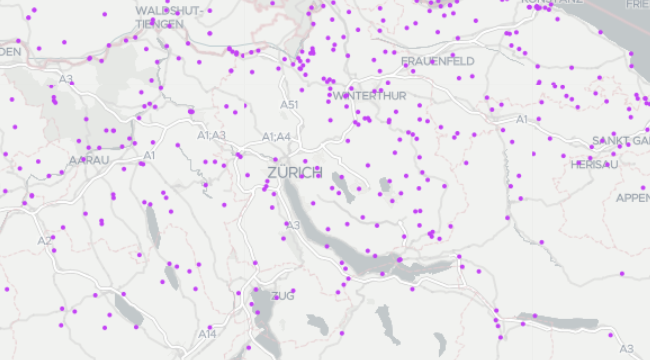
\includegraphics[width=\textwidth]{./Images/ManagementSummary/zurich_tiles.png}
		\caption{Castle Map showcase showing violet dots represented as vector and raster tile data in front of a base map}
	\end{minipage}
	\hfill
	\begin{minipage}[b]{0.48\textwidth}
		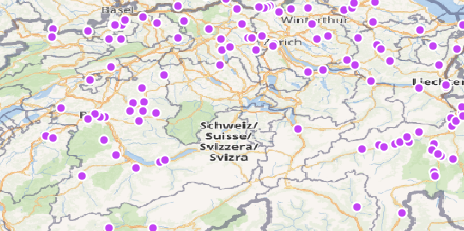
\includegraphics[width=\textwidth]{./Images/ManagementSummary/qgis_wfs3.png}
		\caption{QGIS's experimental WFS3 (OAPIF) vector layer communicating with the API}
	\end{minipage}
\end{figure}
\newpage
\section*{Future Outlook}
The current version of this application can be successfully used to run a WFS/OGC client in tandem with.
Something that would maybe improve the application is to introduce async methods in the API calls, but that is not necessary for now.\\
Another thing would be implementing all the API endpoints (optional ones too) from the OGC - API Features standard.\\
Another interesting extension for the application would be the implementation of the collection \textit{SPATIAL EXTENT} in order to determine the correct location of the features in space. This extension would be very useful for clients who use the API and especially for QGIS.\\
Also, in the future, this application might be benchmarked for performance, comparing it to the existing API that the Castle Map showcase uses in order to assert which one delivers better performance.
\addtocontents{toc}{\protect\setcounter{tocdepth}{1}}